% !Mode:: "TeX:UTF-8:Main"
% arara: pdflatex
% arara: pdflatex
% arara: convert: {density: 160, otheroptions: -dispose previous -delay 10 -loop 1, format: gif}
\documentclass{beamer}

\usepackage{tikz}
\usepackage{bbold}
\usepackage{fourier}
\usetikzlibrary{overlay-beamer-styles}
\setbeamertemplate{navigation symbols}{}

\usepackage{tikzducks}

\begin{document}

\begin{frame}[plain,label=thesis]
\begin{tikzpicture}[remember picture,overlay]
	
% Background image
\node[at=(current page.center)]{%
	\includegraphics[height=\paperheight]{P_Bienio}
};	
%https://commons.wikimedia.org/wiki/File:P_Bienio.jpg
\end{tikzpicture}

\vspace*{1cm}
\begin{tikzpicture}[remember picture, overlay]

% confetti
\node at ({5.4+cos(\thepage)},{28.8-0.0972*(\thepage)}) {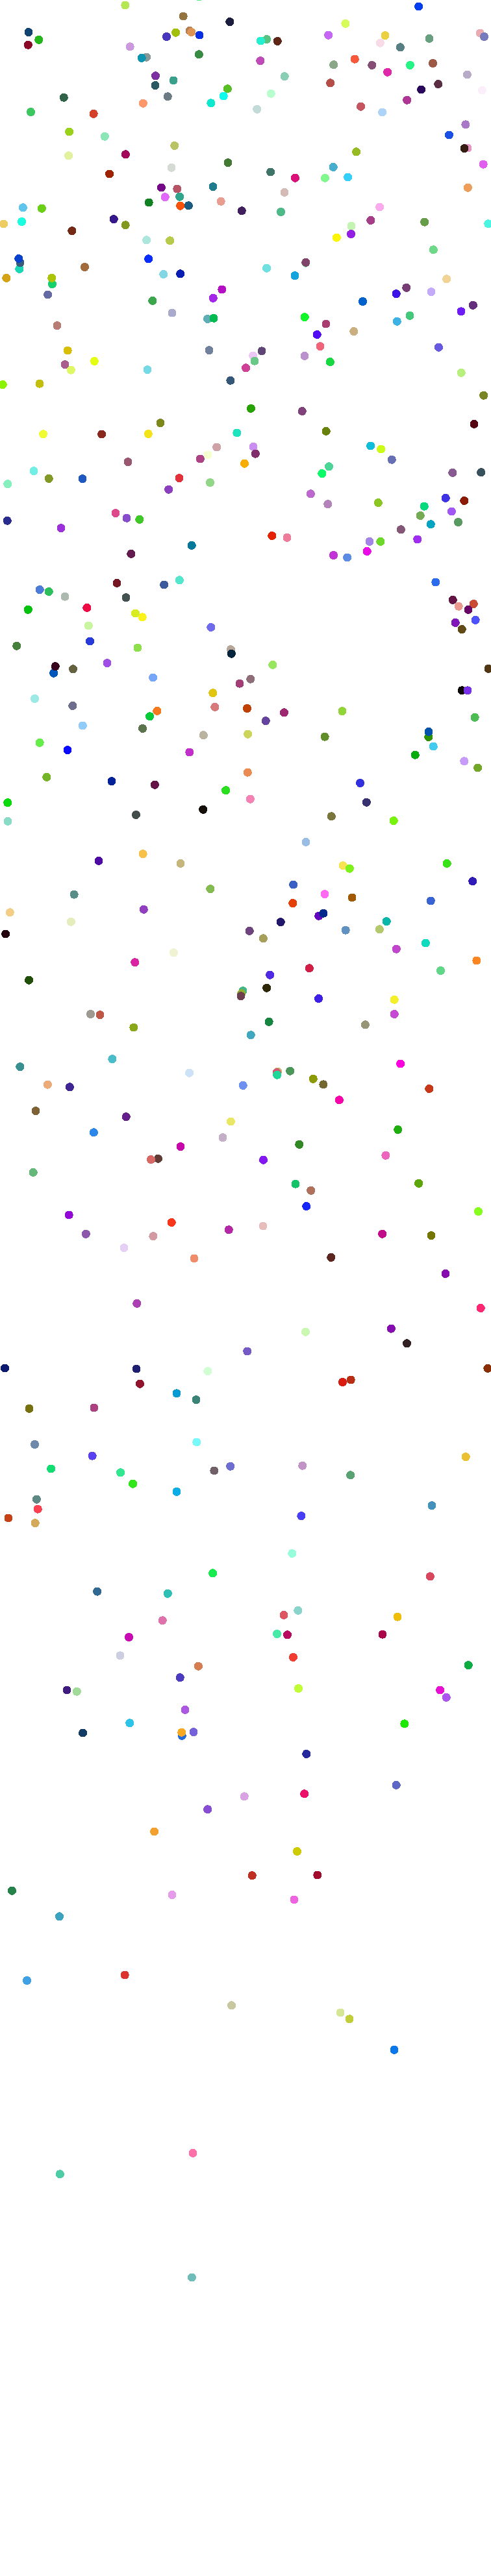
\includegraphics[width=\paperwidth,page=1]{confetti}};

\foreach \x in {0,5,...,1800}{
\only<+>{
		
	% string between duck and ballon
	\draw[gray,thick]
	(2.3, 0.6) .. controls
	(2.3, 0.6) and
	(2.5, -2) ..
	(5.2, {sin(\x)-1.5});
	
	% jumping duck
	\begin{scope}[yshift=sin(\x)*1cm]
		\duck[cap,cricket,xshift=4.8cm,yshift=-2.8cm]
	\end{scope}	
	
}}

% ballon
\shade[ball color=red] (2.3,1.4) ellipse (0.5 and 0.9);
                
% confetti
\node at ({5.4+sin(\thepage)},{28.8-0.0972*(\thepage)}) {\includegraphics[width=\paperwidth,page=2]{confetti}};
                
\end{tikzpicture}
\end{frame}     

%\againframe{thesis}
\end{document} 